\begin{myposter}{
    Обзор
}

    \headerbox
    {Омни-колеса и экипажи}
    {name=first,column=0,row=0,span=3}
    {
        \vspace{-5pt}
        \begin{figure}[H]
            \centering
            \minipage{0.4\textwidth}
                \centering
                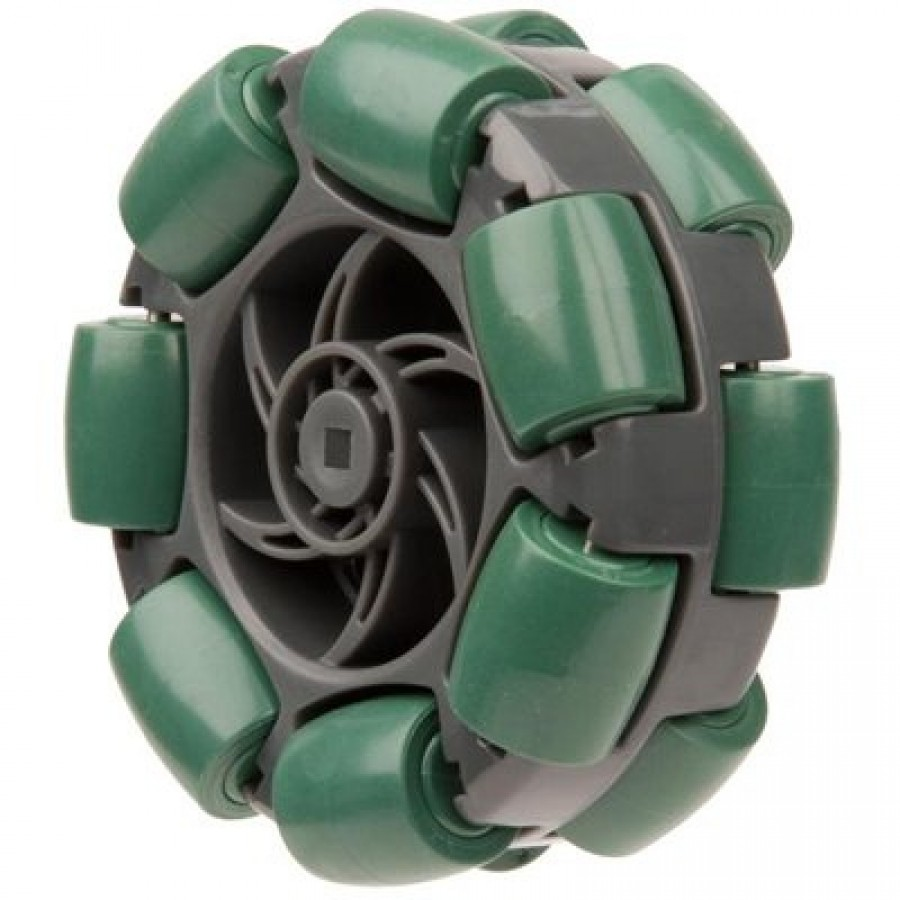
\includegraphics[width=\linewidth]{content/pic/photo/wheel_two_rows.jpg}
            \endminipage
            \minipage{0.5\textwidth}
                \centering
                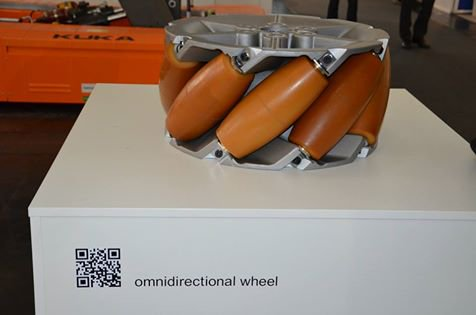
\includegraphics[width=\linewidth]{content/pic/photo/wheel_mecanum.jpg}
            \endminipage
        \end{figure}
        \vspace{-10pt}
        \begin{figure}[H]
            \centering
            \minipage{0.25\textwidth}
                \centering
                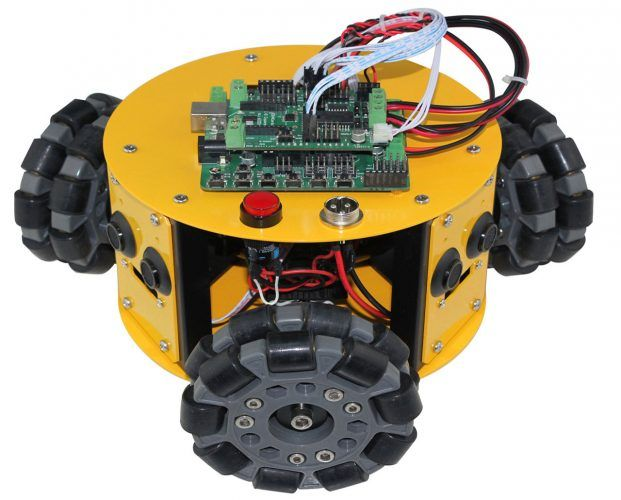
\includegraphics[width=\linewidth]{content/pic/photo/vehicle_three_two_row.jpg}
            \endminipage
            \minipage{0.75\textwidth}
                \centering
                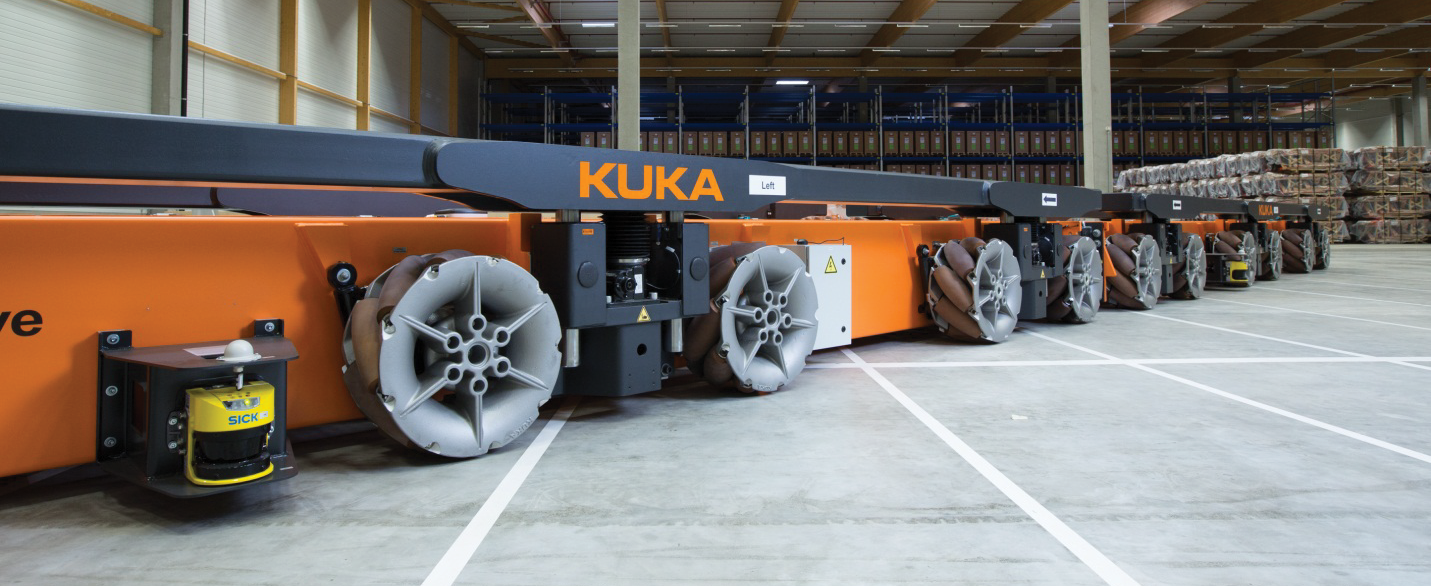
\includegraphics[width=\linewidth]{content/pic/photo/vehicle_kuka.png}
            \endminipage
        \end{figure}
    }
    
    \vspace{50pt}
    \huge{Динамика роликонесущего экипажа с учетом инерции роликов и трения}
    \Large{Кирилл Герасимов}
    
\end{myposter}
